%%%%%%%%%%%%%%%%%%%%%%%%%%%%%%%%%%%%%%%%%%%%%%%%%%%%%%%%%%%%%%%%%%%%%%%%
%                                                                      %
%     File: Thesis_Appendix.tex                                        %
%     Tex Master: Thesis.tex                                           %
%                                                                      %
%     Author: Andre C. Marta                                           %
%     Last modified : 21 Jan 2011                                      %
%                                                                      %
%%%%%%%%%%%%%%%%%%%%%%%%%%%%%%%%%%%%%%%%%%%%%%%%%%%%%%%%%%%%%%%%%%%%%%%%

\setcounter{page}{1}
\chapter{Printed Box Technical Drawings}
\label{annex:drawings}
\begin{figure}[!htb]
  \centering
  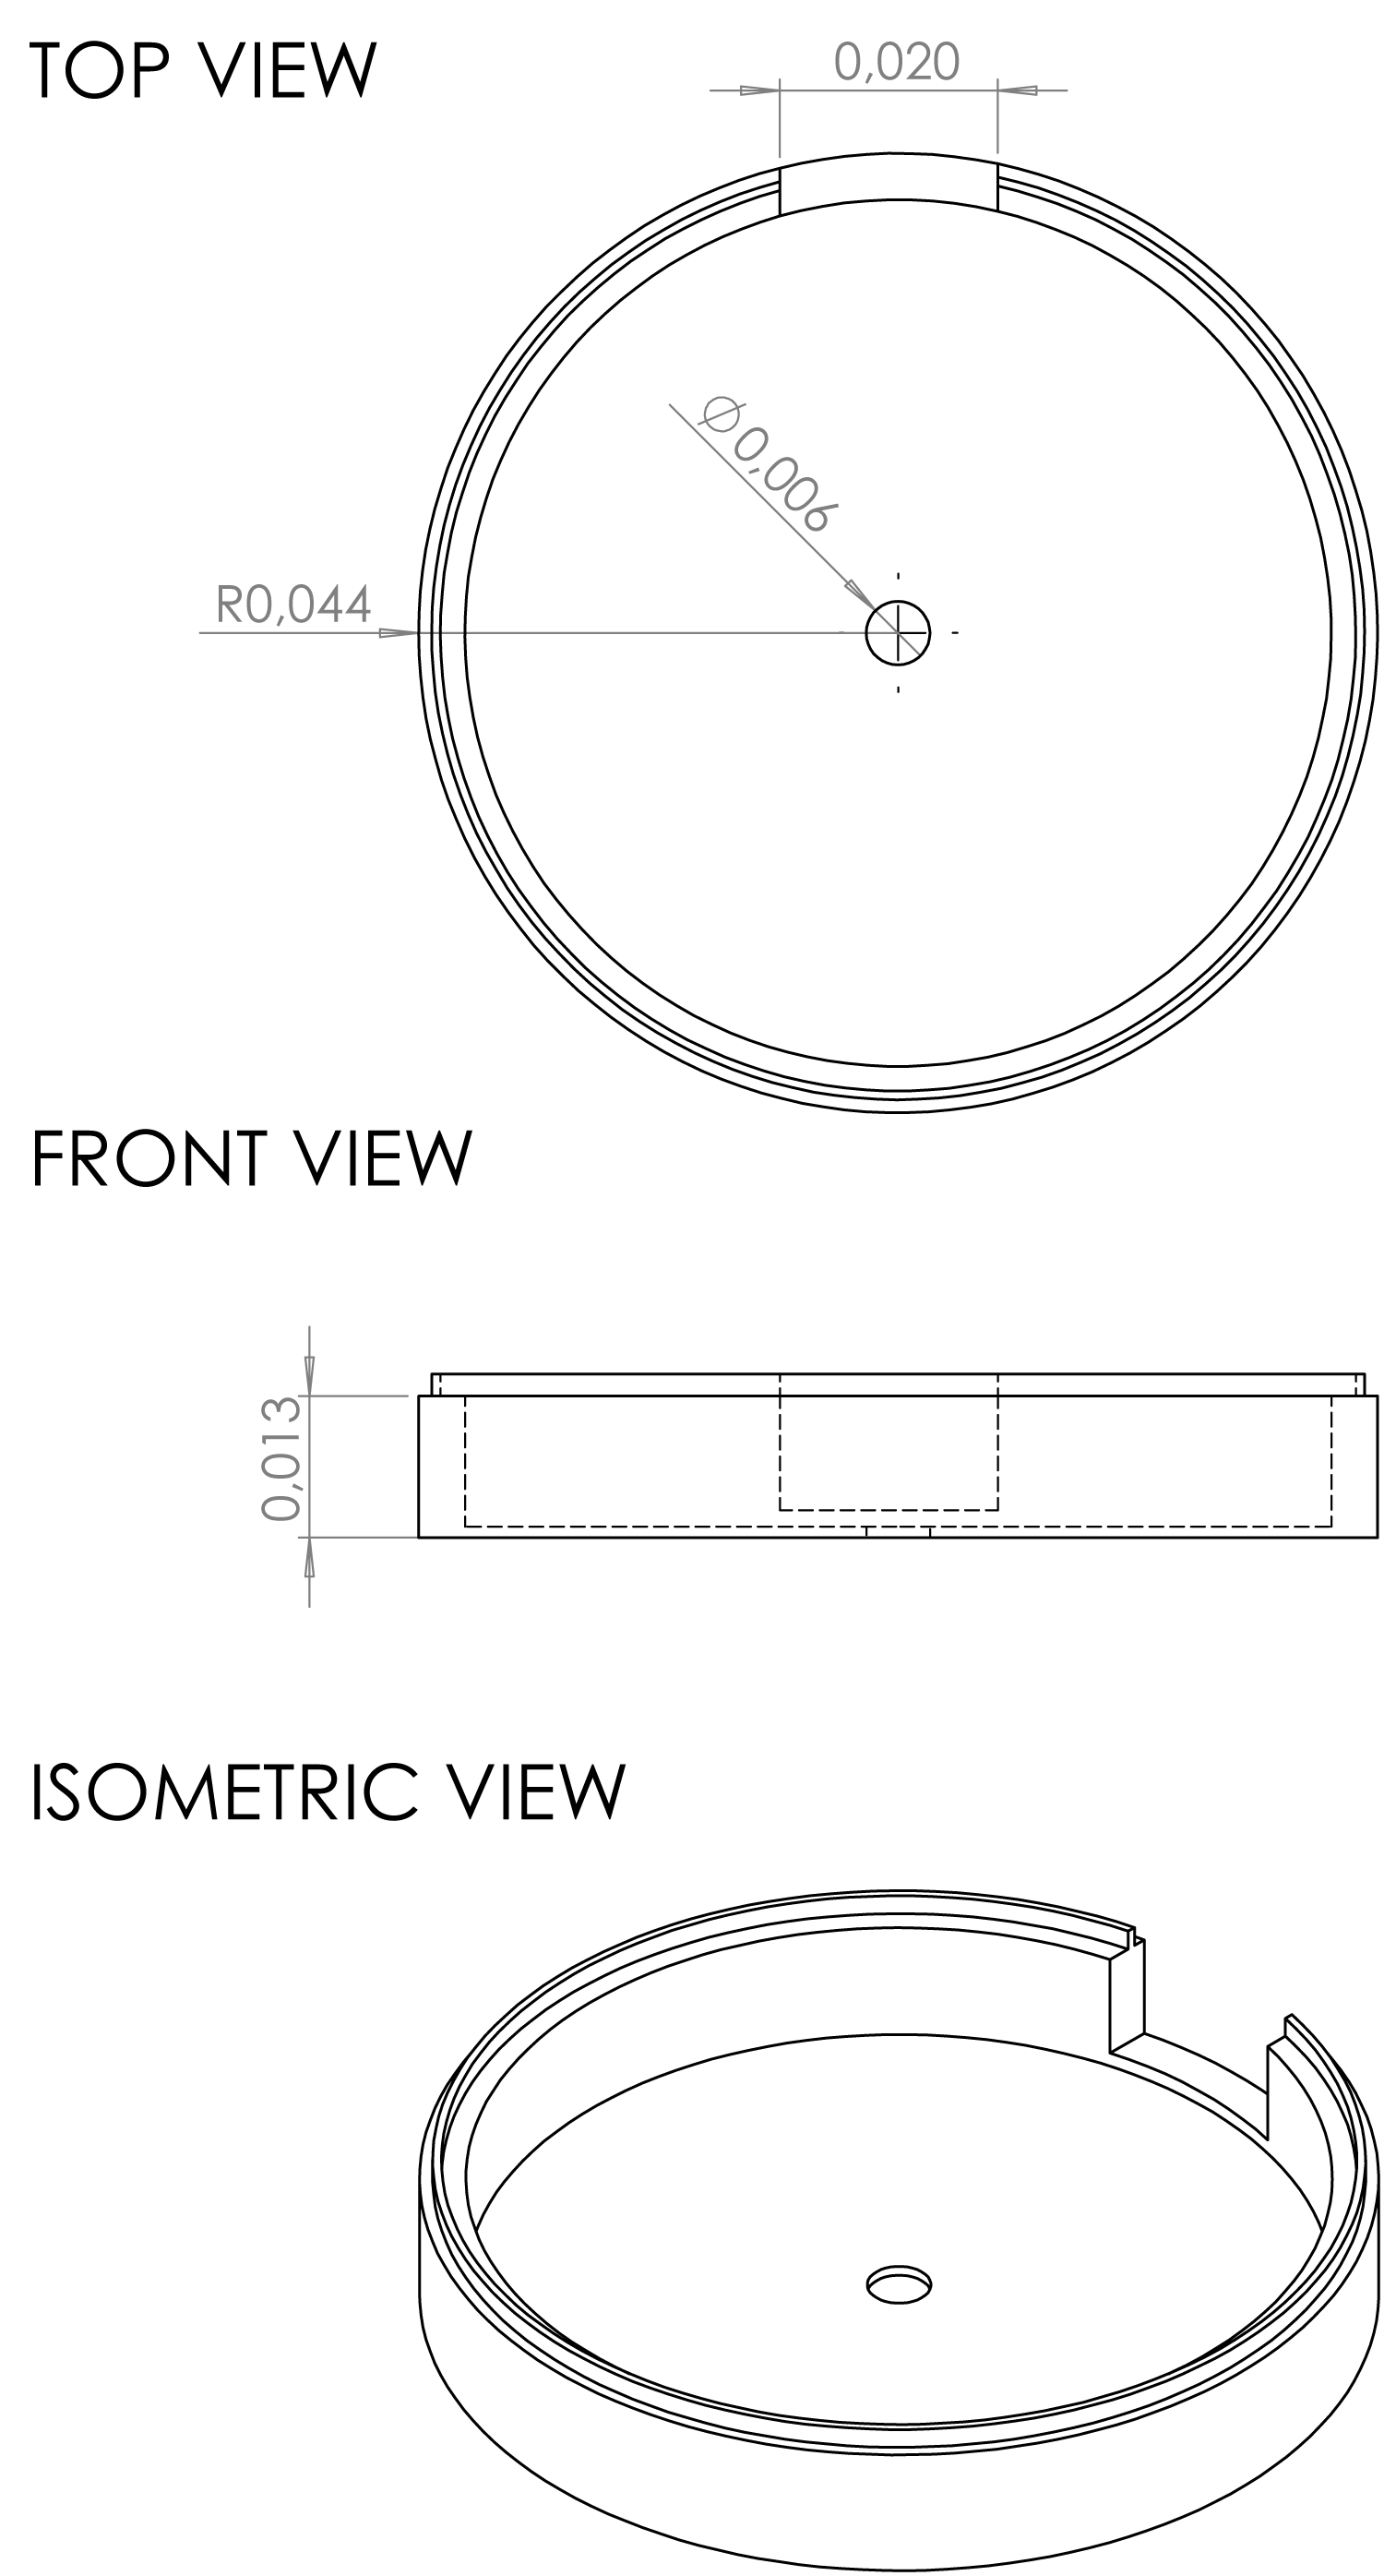
\includegraphics[width=0.8\textwidth]{Figures/Part1.png}
  \caption[Technical Drawing of Printed Box's First Part]{Technical drawing of printed box's first part}
\end{figure}
\begin{figure}[!htb]
  \centering
  \includegraphics[width=0.8\textwidth]{Figures/Part2.png}
  \caption[Technical Drawing of Printed Box's Second Part]{Technical drawing of printed box's second part}
\end{figure}
\begin{figure}[!htb]
  \centering
  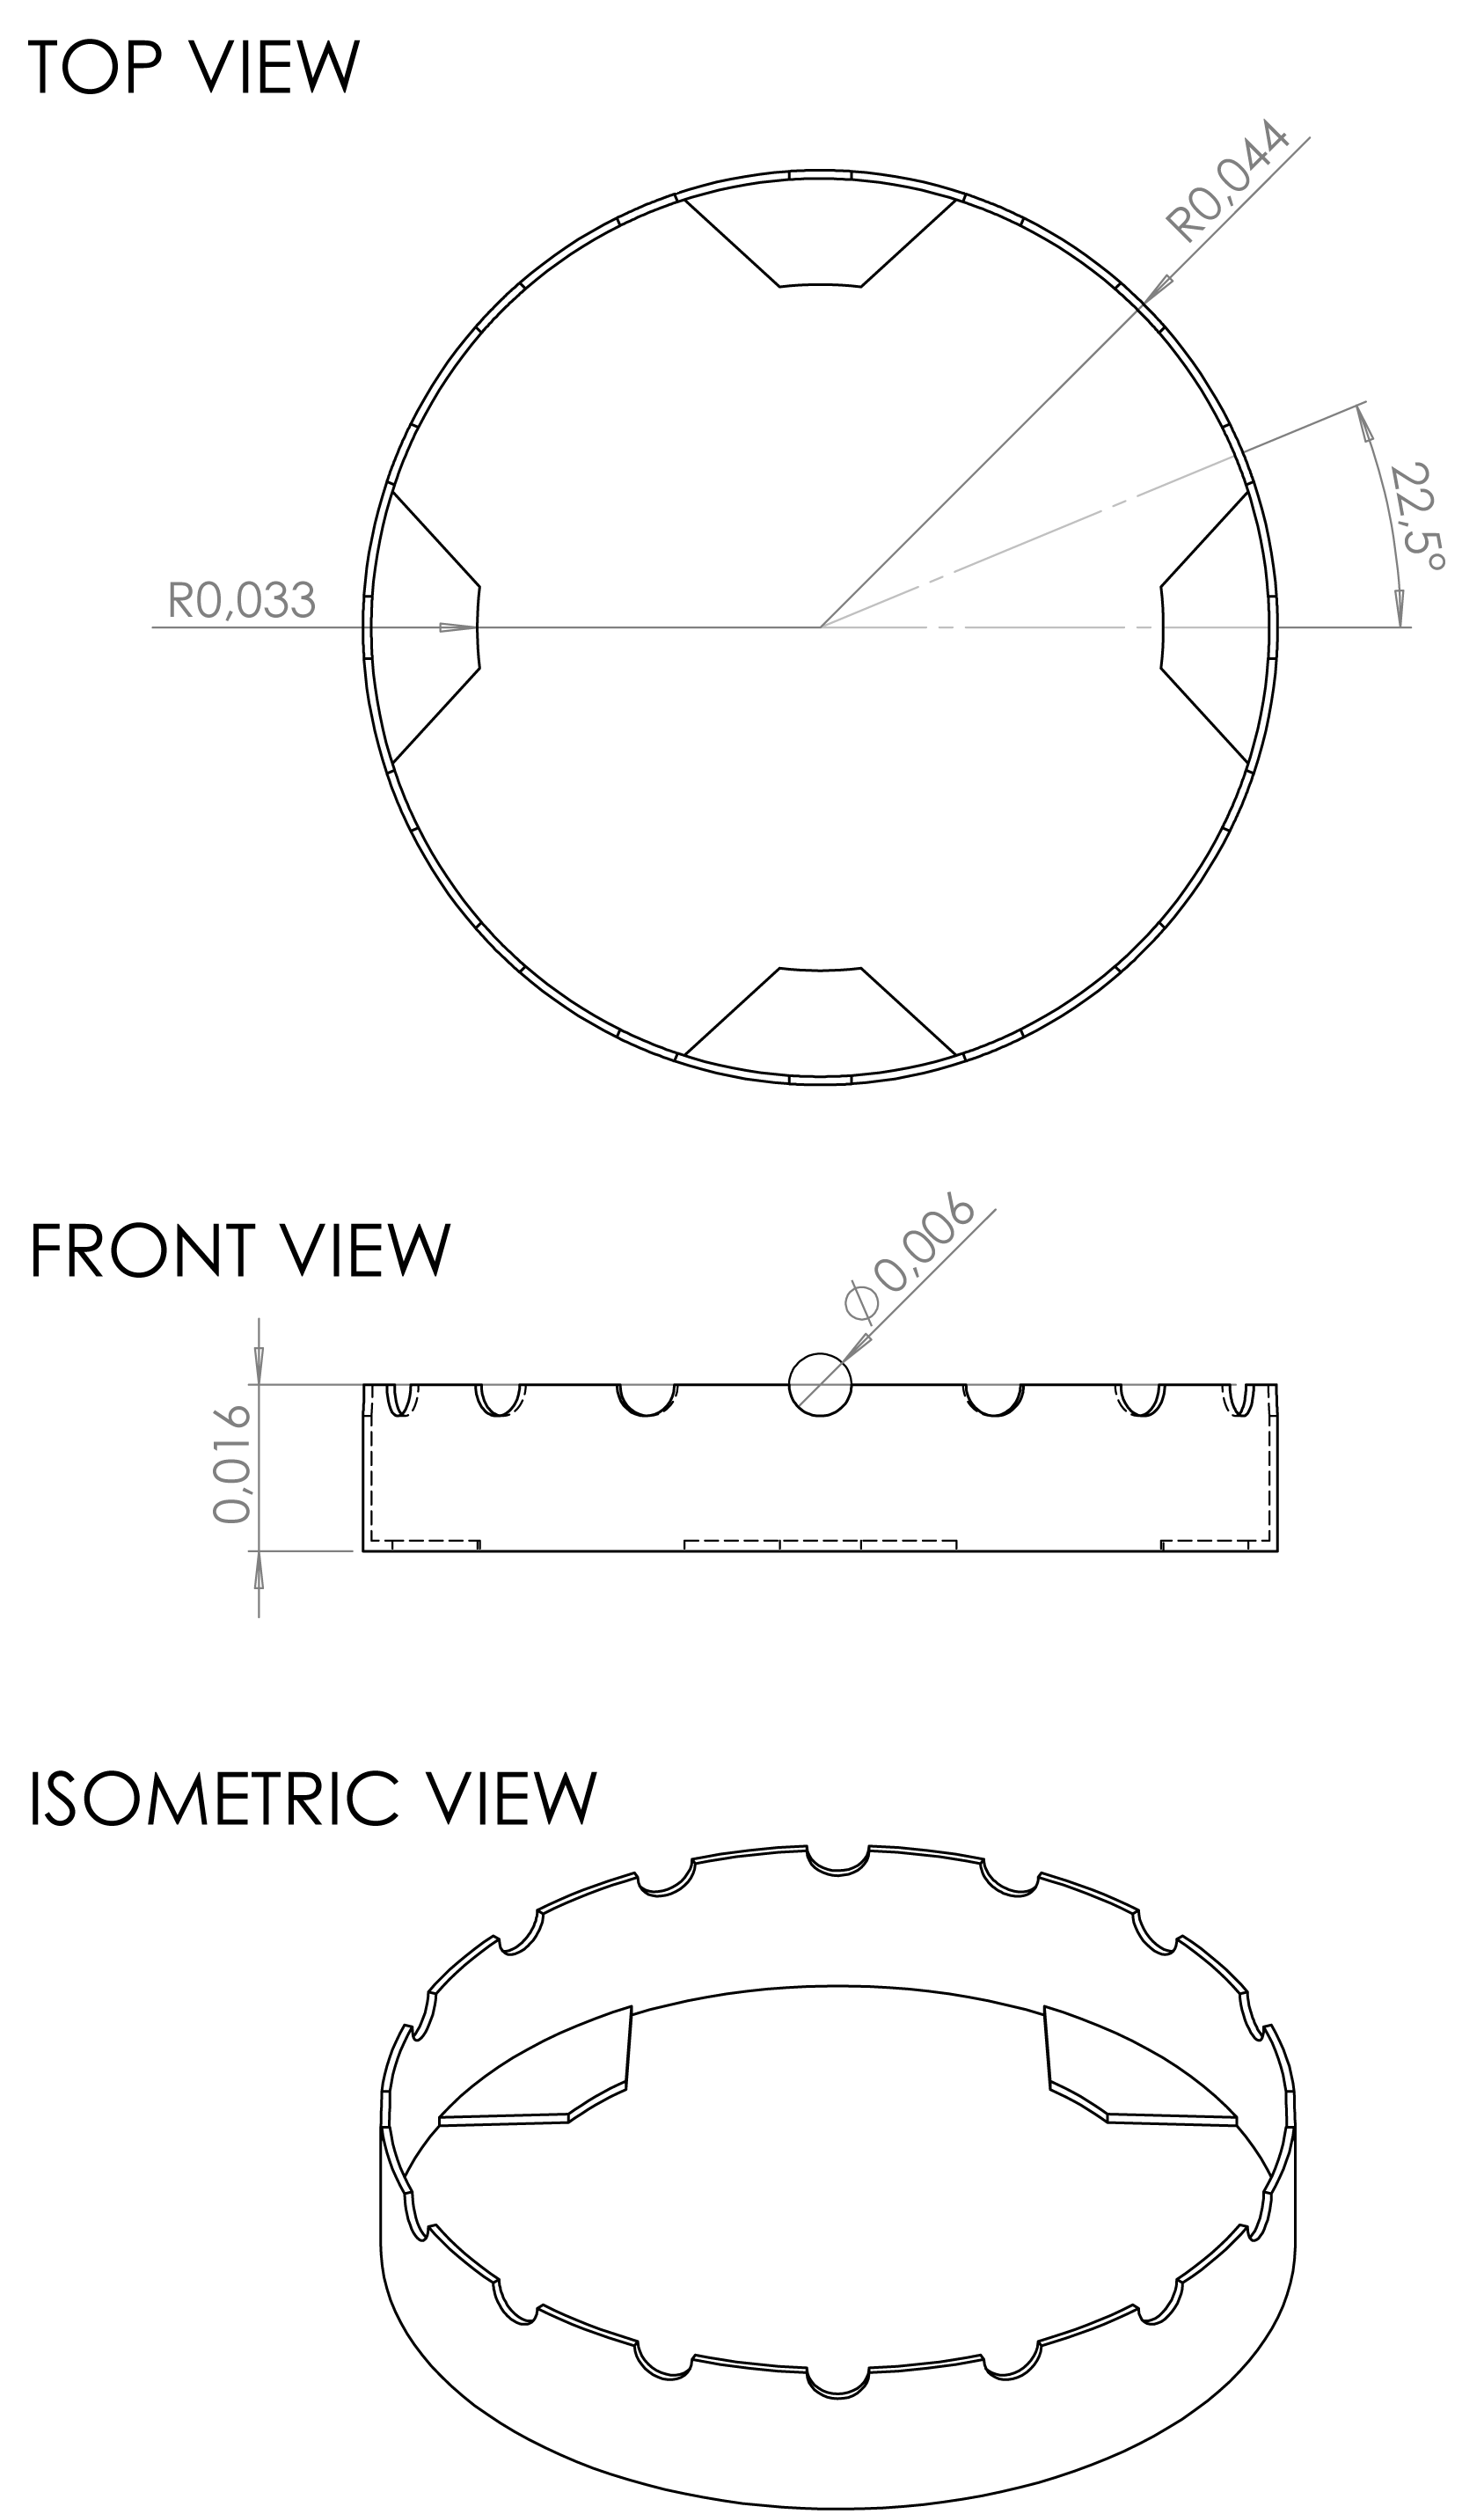
\includegraphics[width=0.8\textwidth]{Figures/Part3.png}
  \caption[Technical Drawing of Printed Box's Third Part]{Technical drawing of printed box's third part}
\end{figure}
\begin{figure}[!htb]
  \centering
  \includegraphics[width=0.8\textwidth]{Figures/Part4.png}
  \caption[Technical Drawing of Printed Box's Fourth Part]{Technical drawing of printed box's fourth part}
\end{figure}
\chapter{Test Procedures}
\section{Visual Material Test}
\label{visualmaterial}
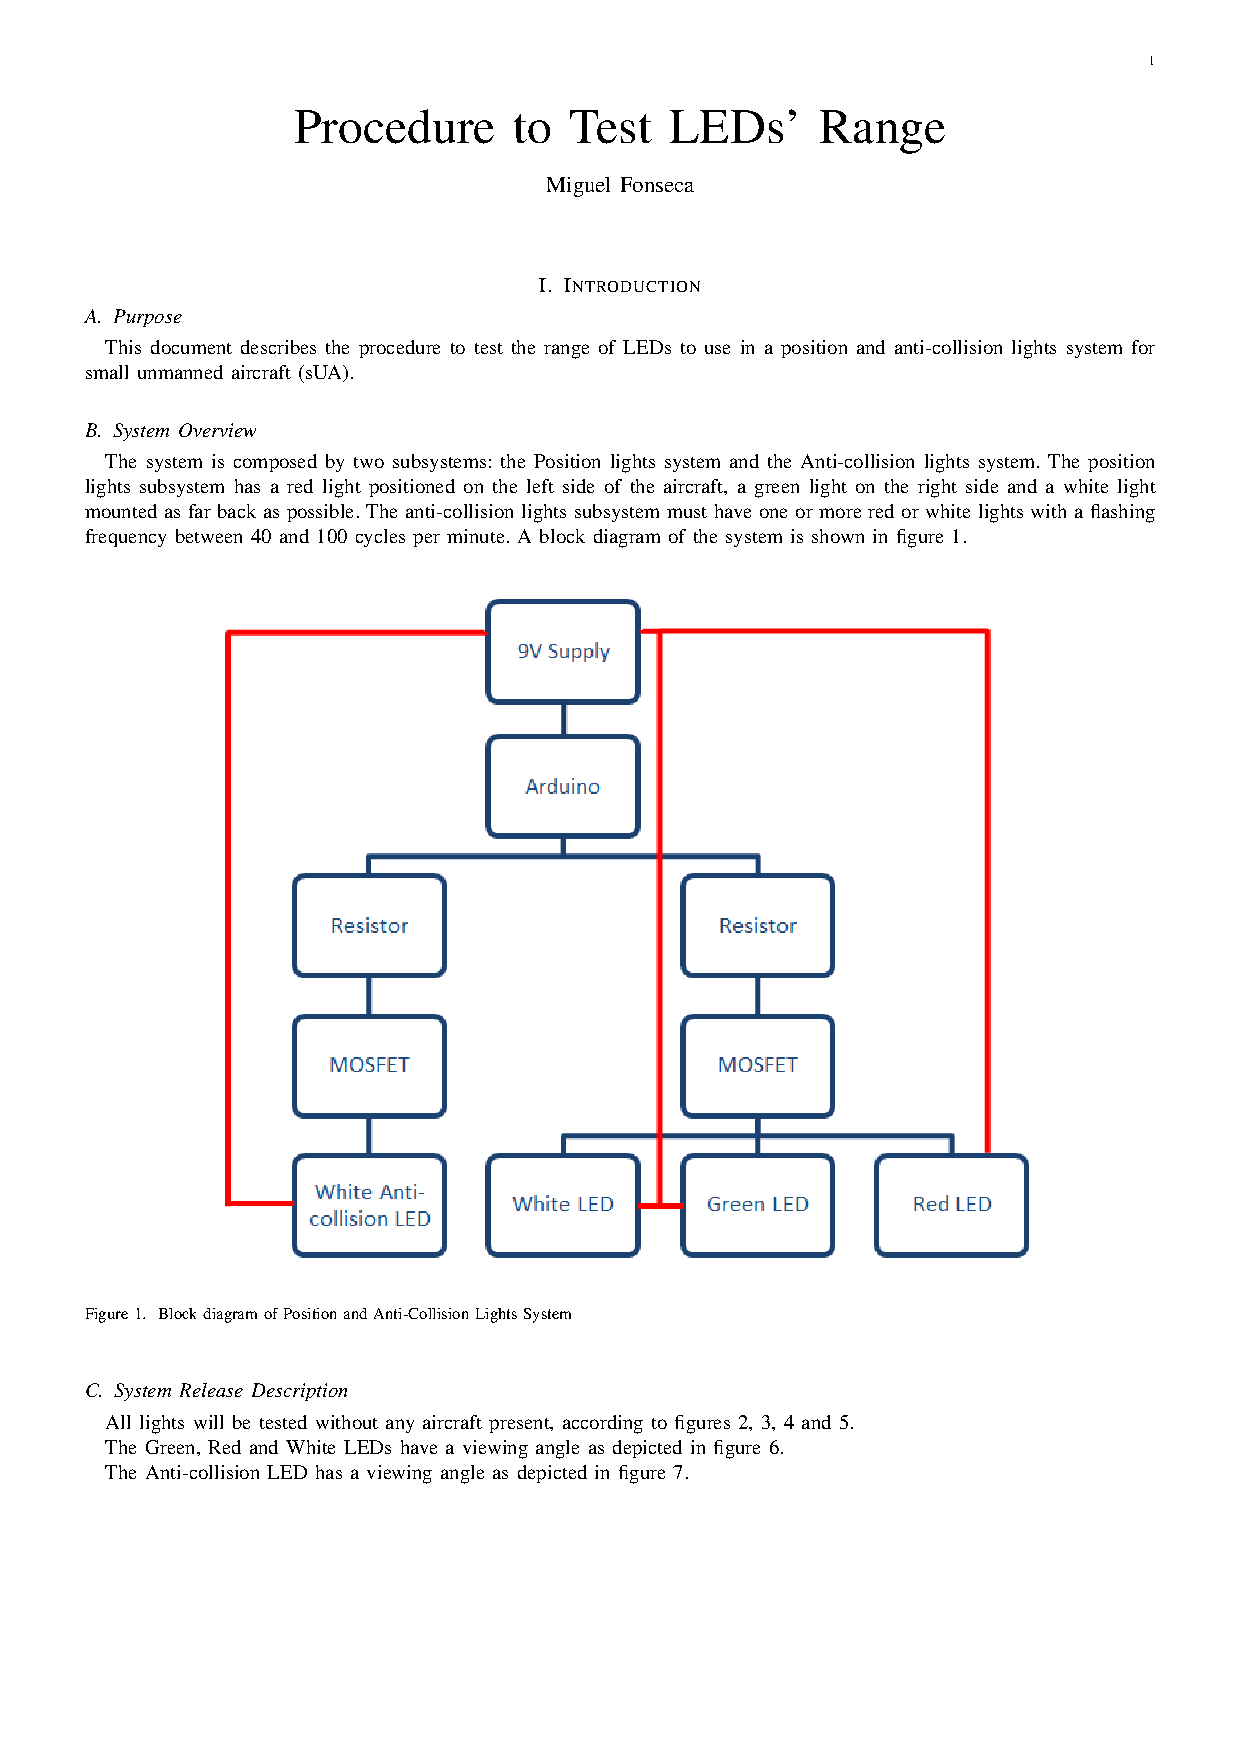
\includepdf[pages={1-}]{testprocedure.pdf}

\section{IR Material Test}
\label{annex:irmaterial}
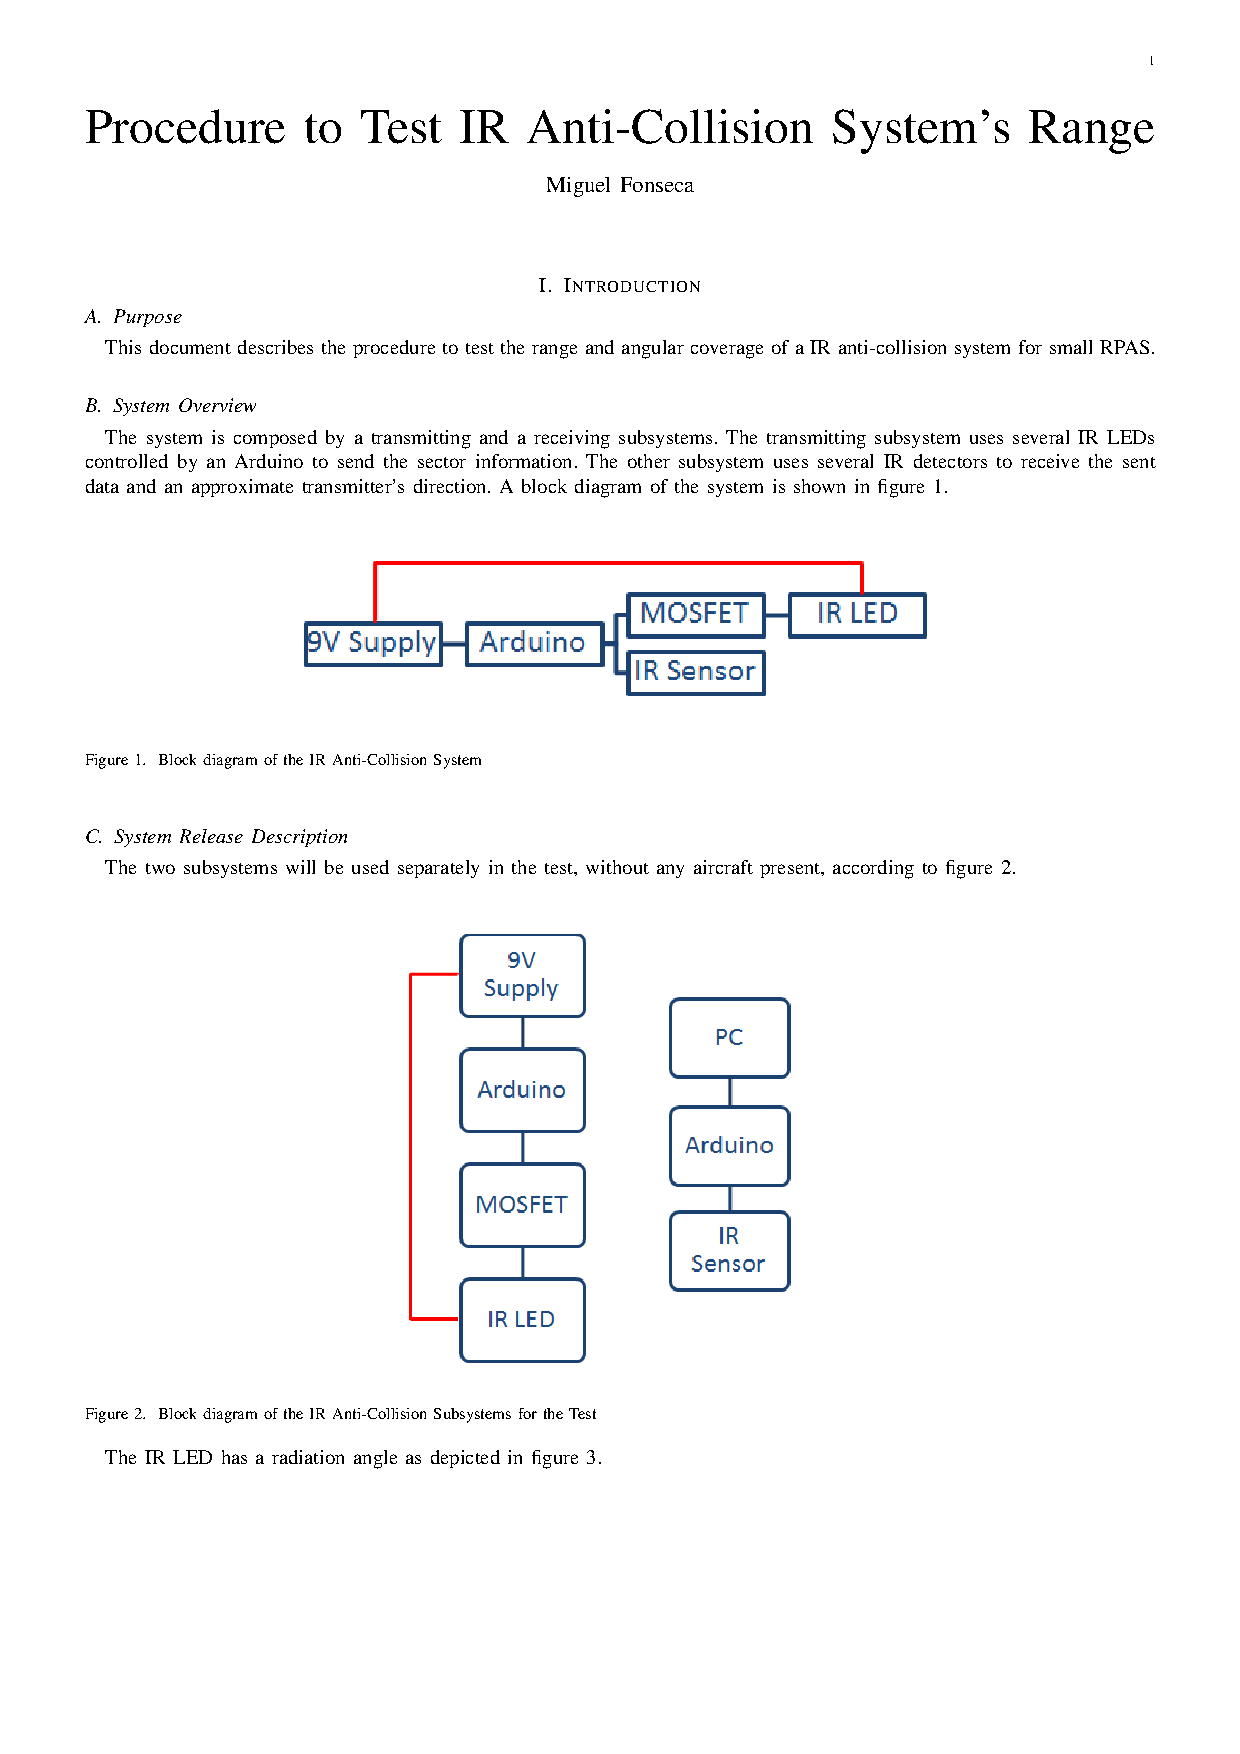
\includepdf[pages={1-}]{testprocedureIR.pdf}

\section{IR Maneuvers Test}
\label{annex:maneuvers}
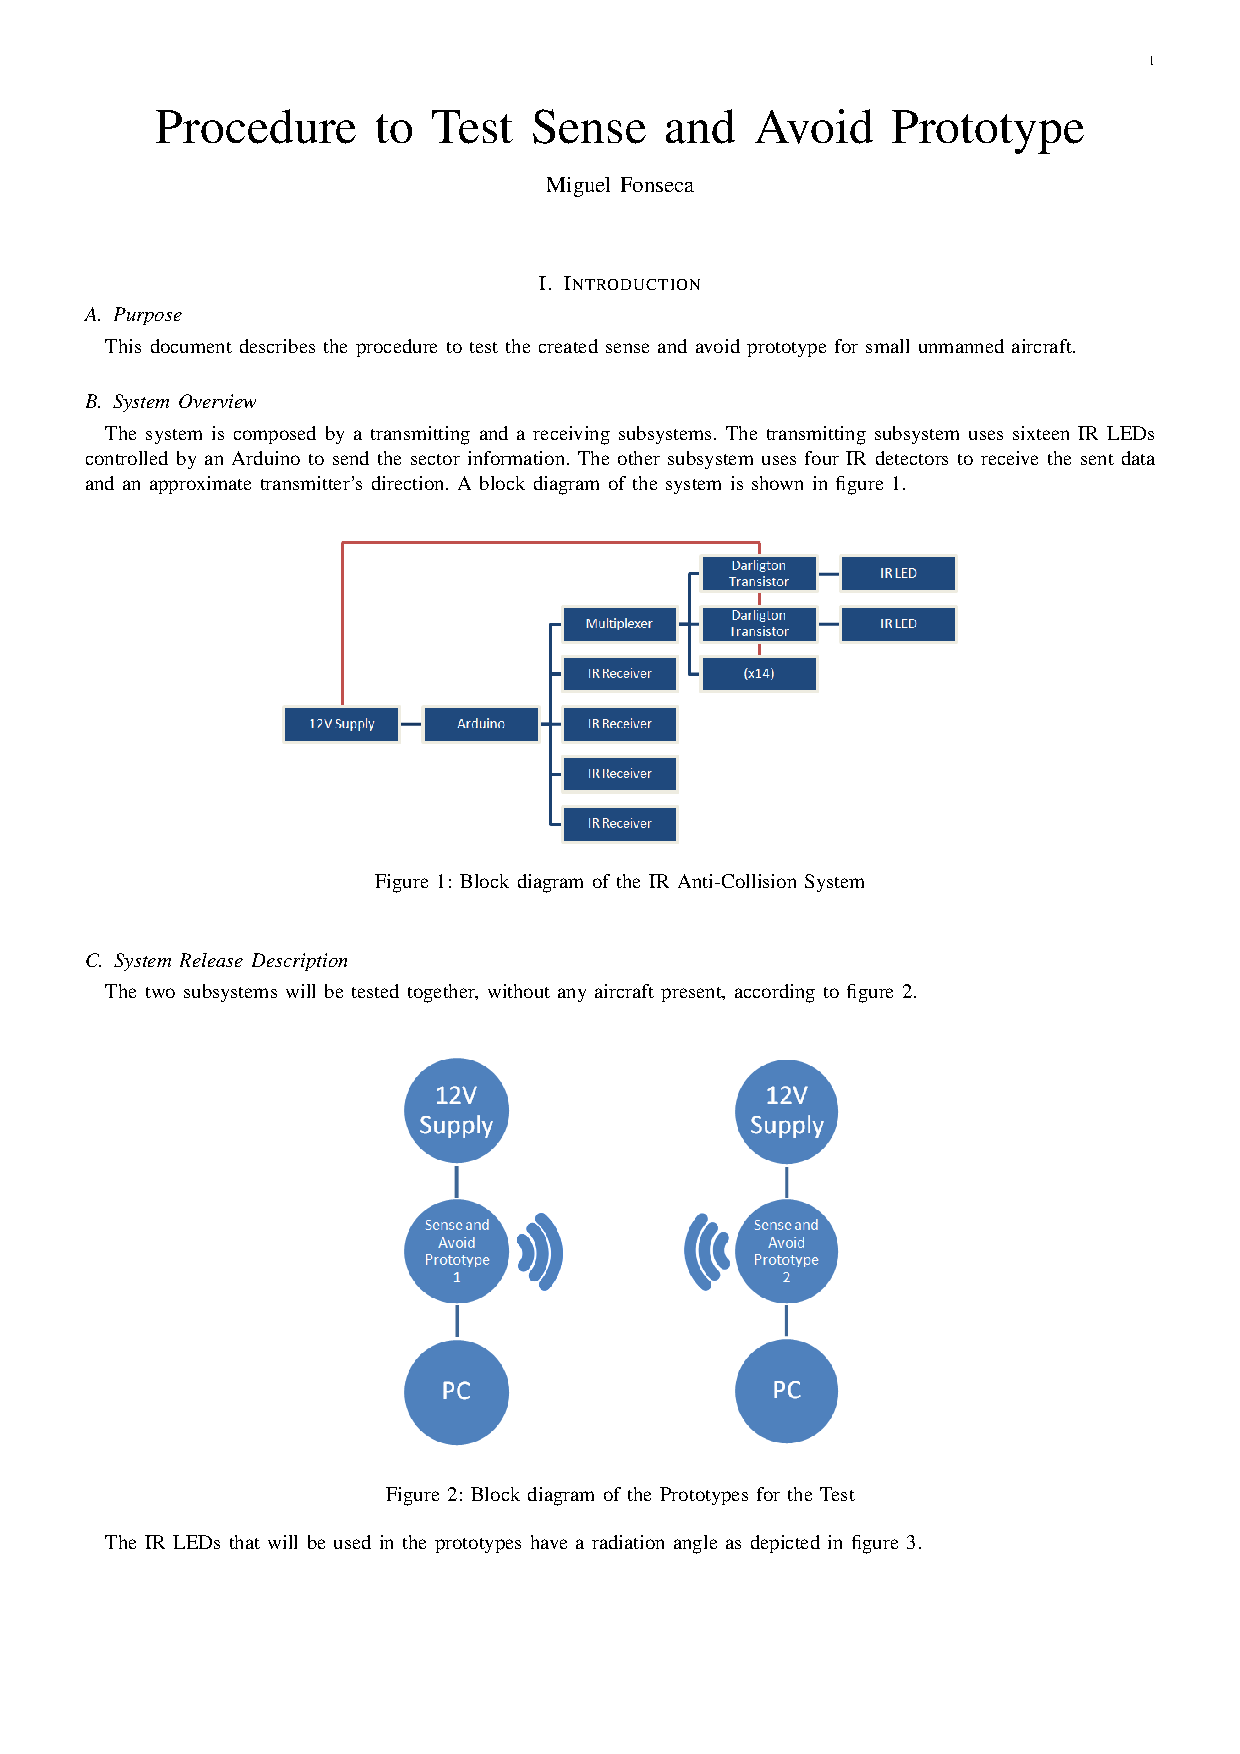
\includepdf[pages={1-}]{testprocedurePrototype.pdf}

\section{IR Sense and Avoid Test with Aircraft}
\label{annex:sas}
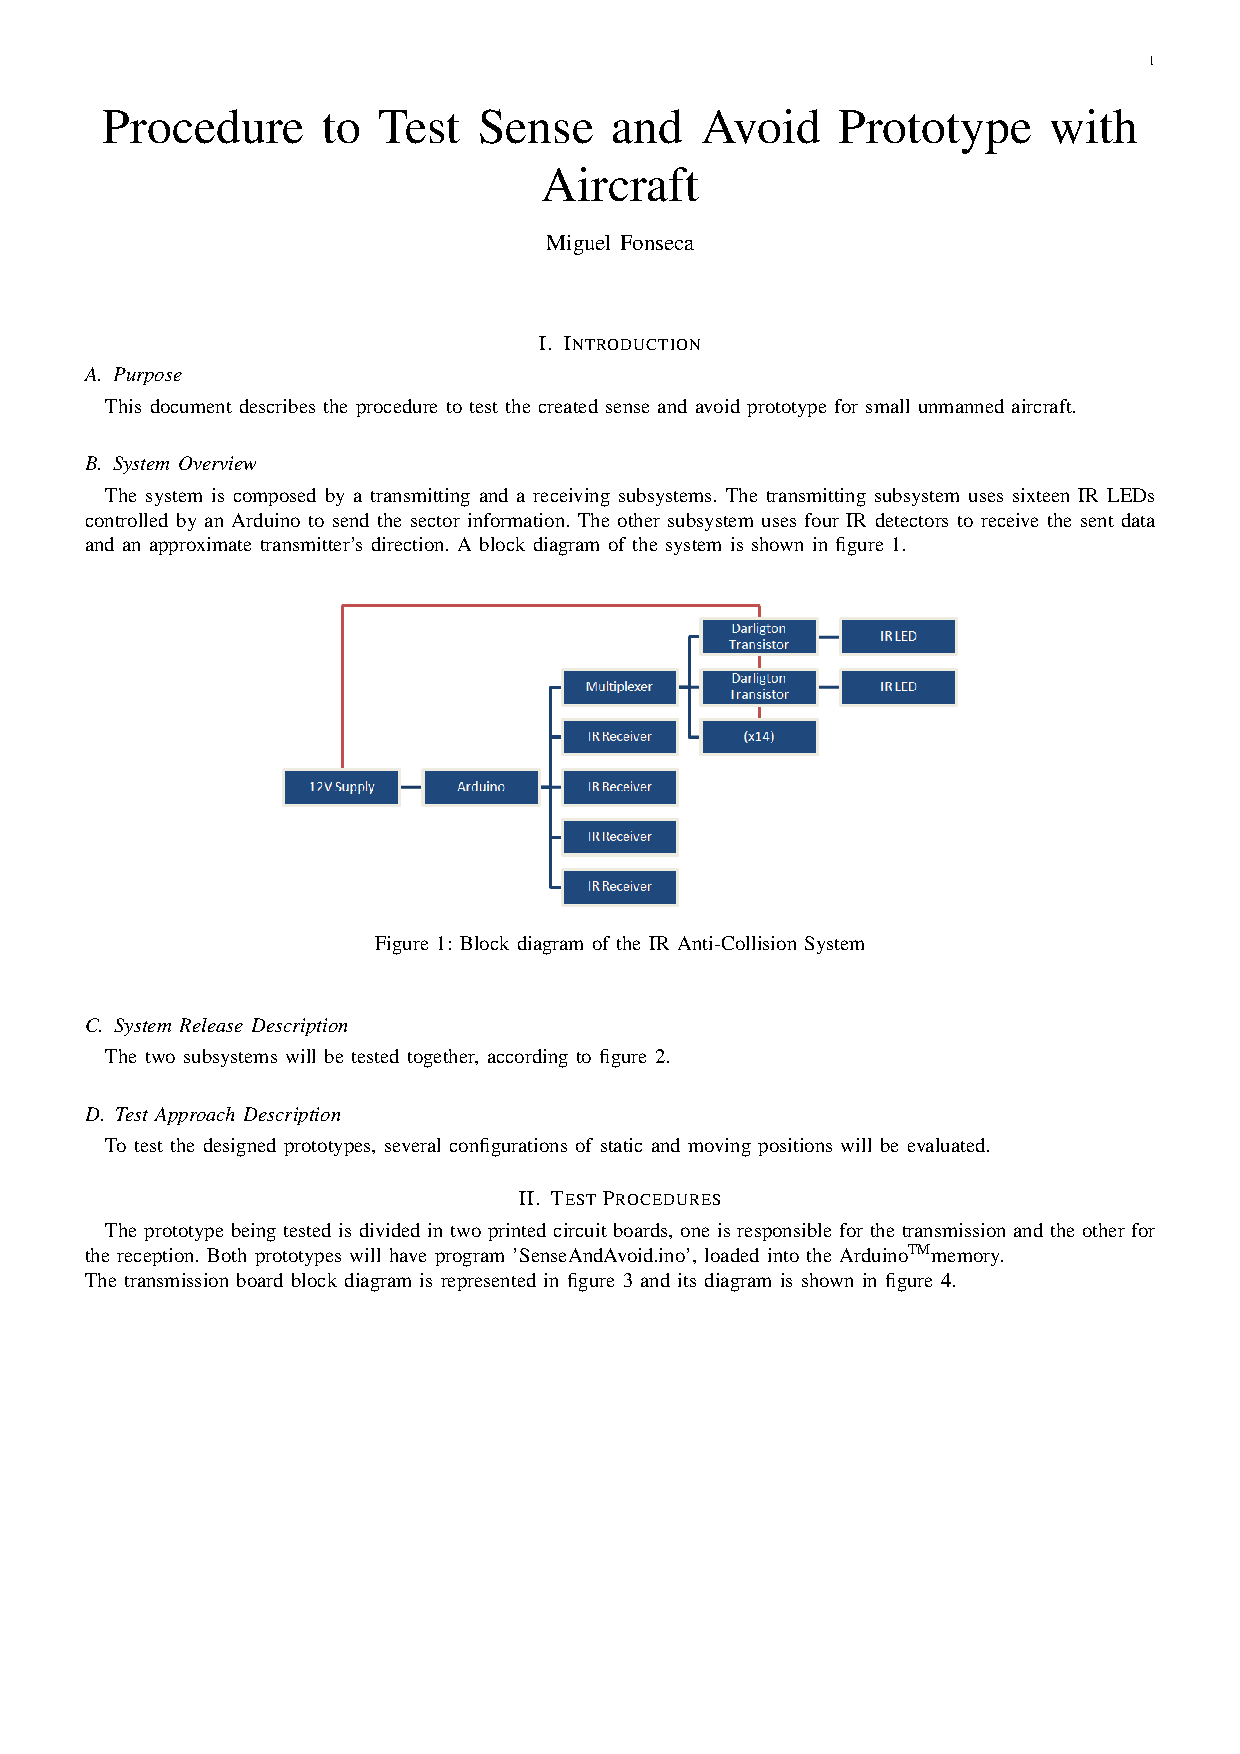
\includepdf[pages={1-}]{testprocedureAircraft.pdf}



%% ----------------------------------------------------------------------
%\section{Vector identities}
%\label{section:vectorIdentities}
%
%\begin{equation}
%	\nabla \times \left( \nabla \phi \right) = 0
%	\label{eq:cross_nnp}
%\end{equation}
%
%\begin{equation}
%	\nabla \cdot \left( \nabla \times {\bf u} \right) = 0
%	\label{eq:dotCross_nnu}
%\end{equation}
%
%\cleardoublepage

